\label{monitoramento_servicos}

Neste capítulo são apresentadas informações decorrentes da arquitetura de monitoramento de serviços e da realização do monitoramento do barramento de serviços por meio do protocolo \acrshort{SNMP}. Na Seção \ref{arquitetura_monitoramento} é apresentado o conceito da arquitetura de monitoramento de serviços. Na Seção \ref{recursos_monitoramento} é descrito o monitoramento dos recursos do barramento de serviços. Na Seção \ref{integracao_snmp} são discutidos detalhes do funcionamento do protocolo \acrshort{SNMP}. Na Seção \ref{metricas_monitoramento} são expostas as definições e escolhas das métricas adotadas para a realização do monitoramento do barramento de serviços. Na Seção \ref{instrumentacaoErlangms} são descritos argumentos para instrumentação do para a coleta dos dados para a realização do monitoramento.

\section{Arquitetura de Monitoramento de Serviços}%
\label{arquitetura_monitoramento}

A arquitetura de \textit{software} é um conceito ou modelo de organização de uma estrutura, essa estrutura pode ser um módulo ou componentes de \textit{software}. De acordo Shaw e Garlan \cite{garlan1993introduction}, um estilo arquitetônico, pode definir um grupo sistemas com organização estrutural. Estilo arquitetônico determina componentes e conectores que são utilizados, com conjuntos de restrições, essas restrições podem ser topológicas. Nesse seguimento Clements \textit{et al.} \cite{clements2002documenting} descreve, a arquitetura de \textit{software} de um sistema é o conjunto de estruturas necessárias para entender o \textit{software}, que inclui elementos, relações entre eles e suas propriedades.

A arquitetura para o monitoramento de serviços tem como objetivo estabelecer a integração entre o barramento de serviços e ferramentas de monitoramento por meio de um agente de monitoramento. Para isso foi selecionada uma visão arquitetural da categoria \textit{Runtine}, que apresentam os componentes e suas interações em tempo de execução. Segundo Clements \textit{et al.} \cite{clements2002documenting}, uma visão é uma representação de uma estrutura, e afirma uma visualização é uma representação de um conjunto de elementos do sistema e a relação entre eles. Nesse seguimento foram definidos os seguintes componentes:

\begin{itemize}
    \item \textbf{Barramento de serviços} - Provedor de informações e dados, a partir do seu funcionamento, contempla o componente \textbf{\textit{\acrshort{ESB}}}; 
    \item \textbf{Ferramenta de monitoramento} - Coletor de informações e dados para realizar o monitoramento e provedor de informações sobre o funcionamento de serviços e aplicações; 
    \item \textbf{Agente de monitoramento} - Coletor de informações e dados de monitoramento, armazena informações e dados de monitoramento e coletados pelo agente de monitoramento. Transmite informações e dados de monitoramento para a ferramenta de monitoramento, abrange o componente \textbf{Banco de Dados}
\end{itemize}

Com a definição da arquitetura de monitoramento de serviço e a organização de seus componentes espera-se obter níveis baixos de dependência entre as soluções. Os componentes implementados podem ser conectados em outras aplicações. Na arquitetura definida deste trabalho o meio de comunicação entre os componentes é feito por meio de integração, que possibilita manter um nível baixo de dependência das aplicações e a mudança de barramento de serviços ou da ferramenta de monitoramento, sem prejuízo à arquitetura e ao funcionamento da monitoramento de serviços. O modelo conceitual da arquitetura pode ser visualizado na figura \ref{fun:fig:arquitetura_conceitual_monitoramento}

\begin{figure}[H]
	\begin{center}
	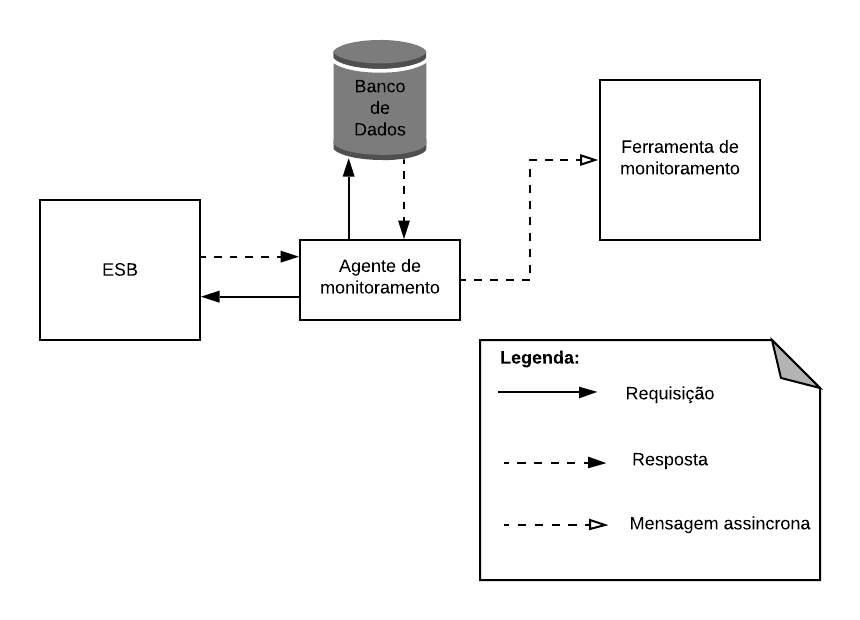
\includegraphics[scale = 0.90]{img/Arquitetura_Proposta_Monitoramento.png}
		\caption{Arquitetura conceitual para o monitoramento de serviços.}
		\label{fun:fig:arquitetura_conceitual_monitoramento}
	\end{center}
\end{figure}

Como parte da arquitetura o barramento de serviços é o componente responsável por gerar dados e informações a partir do seu funcionamento, a partir dessas informações que monitoramento é realizado, outro componente definido na arquitetura é a ferramenta de monitoramento, a ferramenta de monitoramento é responsável por apresentar informações do funcionamento dos serviços monitorados a partir das informações geradas pelo barramento de serviços. Por fim, o componente agente de monitoramento é encarregado de coletar e transmitir as informações geradas pelo barramento de serviços para a ferramenta de monitoramento.  

Neste trabalho os componentes da arquitetura na visão de \textit{runtime}\cite{clements2002documenting} possuem as seguintes descrições:

\subsubsection{Barramento de Serviços}
O barramento de serviços é representado pelo Erlangms que dispõem de uma arquitetura SOA com o estilo arquitetural REST, sua implementação foi feita na linguagem funcional Erlang. O Erlangms é o \acrshort{ESB} utilizado pelo \acrshort{CPD} da \acrshort{UnB} para implementação e modernização de \textit{softwares} na \acrshort{UnB}. O barramento de serviços é utilizado para a integração de várias aplicações heterogêneas por meio de serviços.

\subsubsection{Ferramenta de Monitoramento}
A ferramenta de monitoramento é representado pelo Nagios\textsuperscript{\textregistered} foi projetado para realizar o monitoramento de ativos de rede, sistemas e serviços, notifica os responsáveis pelos ativos de rede, sistema e serviços que estão registrados como contatos emergenciais. A ferramenta é utilizada pelo \acrshort{CPD} da \acrshort{UnB} para o acompanhamento da  disponibilidade de seus serviços.

\subsubsection{Agente de Monitoramento}
O agente de monitoramento é representado pelo Exometer que é um \textit{framework} que executa instrumentação e permiti a exportação de dados, foi implementado em Erlang. Neste trabalho foi utilizado o módulo SNMP da ferramenta para realizar a integração do barramento de serviços e a ferramenta de monitoramento. Com o agente de monitoramento é possivel criar métricas e grupo de dados para o monitoramento.

\subsubsection{Comunicação}

A mensagens trocadas entre os componentes barramento de serviços e ferramenta de monitoramento com intermediação do Agente de monitoramento é feita por meio do protocolo \acrshort{SNMP}. O protocolo é utilizado na camada de Aplicação do modelo OSI \cite{tanenbaum2003redes}, é responsável pela transmissão de dados e informações de gerenciamento e monitoramento entre dispositivos e ativos de rede. Cabe ressaltar a importância da definição de um protocolo para a comunicação, a escolha de um modelo de comunicação, possibilita a manutenção adequada, a seleção de outras ferramentas que trabalhem com o protocolo e a baixa dependência de aplicações.     

Com o conceito arquitetural definido, está fortemente alinhado com o ambiente computacional da \acrshort{UnB}, este trabalho emprega ênfase na integração dos componentes para a realização do monitoramento.   

\section{Monitoramento dos Recursos do Barramento de Serviços}%
\label{recursos_monitoramento}

O \acrshort{CPD} da \acrshort{UnB} adotou como solução para a modernização, migração dos sistemas e tecnologia a implementação de uma arquitetura orientada a serviços, que vem sendo bastante utilizada principalmente para criação de serviços (\textit{web services}). A implementação dos serviços tem aumentado, devido a flexibilidade definida na arquitetura e o aumento da demanda para a realização de integração de sistemas, além da curva de aprendizagem ser alta. A partir da implementação e disponibilização de  vários serviços, monitorar e acompanhar o funcionamento, tem se tornado uma tarefa que tem demandado um grande esforço das equipes de desenvolvimento do \acrshort{CPD}. 

No \acrshort{CPD}, o monitoramento do barramento de serviços da \acrshort{UnB} é realizado de três formas conhecidas, uma por meio do \textit{Log} de arquivos gerado pelo barramento, outra por meio de serviços (\textit{web services}) providos pelo barramento, além da nativa que é disponibilizada pela empresa que mantém e gerencia a linguagem Erlang.

\subsubsection{Monitoramento do Barramento de Serviços por \textit{Log} de Arquivos}

As informações de registros do \textit{Log} geradas pelo barramentos de serviços, são coletadas e armazenadas. A abordagem utilizada para o acompanhamento do funcionamento do barramento de serviços possibilitou o monitoramento sem a necessidade de modificação no código-fonte do barramento de serviços, observado que um dos motivos pelo acompanhamento por meio do \textit{Log}, é realizar o monitoramento em tempo real sem a perda de desempenho  do barramento de serviços durante o funcionamento. 

As informações armazenadas originárias do arquivo de \textit{Log} são transmitidas e suas métricas apresentadas em um \textit{dashboard}, esse \textit{dashboard} foi desenvolvido para o acompanhamento do funcionamento do barramento de serviços graficamente, como por exemplo o quantitativo de erros por serviço, o \textit{dashboard} com os gráficos de apresentação pode ser visualizado na figura \ref{fun:fig:dashboardS} \cite{filgueirasmonitoramento}.

\begin{figure}[H]
	\begin{center}
	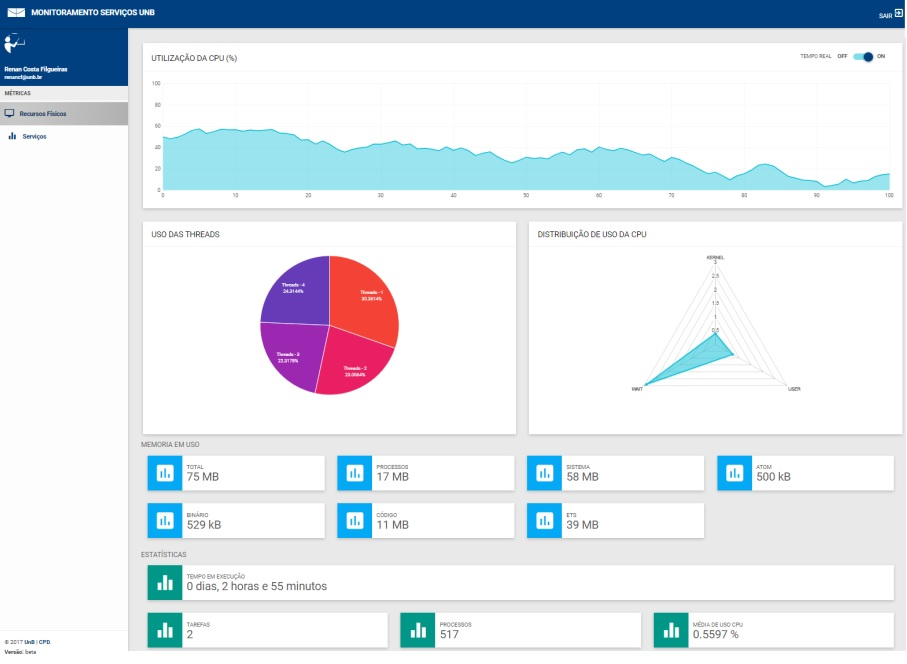
\includegraphics[scale = 0.70]{img/dashboard.jpg}
		\caption{\textit{Dashborad} de monitoramento \cite{filgueirasmonitoramento}.}
		\label{fun:fig:dashboardS}
	\end{center}
\end{figure}

\subsubsection{Monitoramento do Barramento de Serviços por Serviços (\textit{Web Services})}
O barramento de serviços possui em seu código-fonte a implementação de serviços que utilizam módulos Erlang que possibilitam o acompanhamento dos recursos computacionais em que o barramento de serviços está funcionando. 

Esses serviços não dispõem de elementos gráficos, fornecem informações a partir da requisição de um serviços, para a execução desse serviço basta apenas utilizar a \acrshort{URL} do serviço específico e uma ferramenta de testes de \acrshort{API}, que possibilita a obtenção das informações requisitadas. As informações retornadas a partir do serviço por meio de uma requisição pode ser visualizada na figura \ref{fun:fig:memoriaEMS}.

\begin{figure}[H]
	\begin{center}
	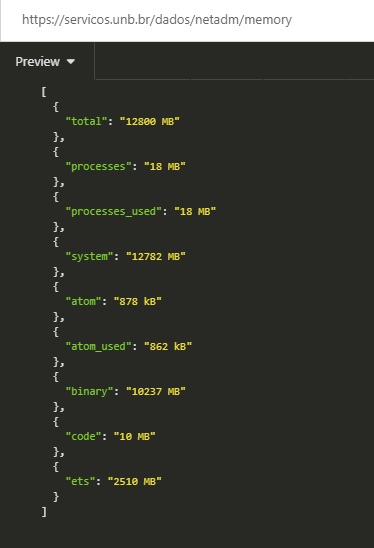
\includegraphics[scale = 0.90]{img/monitoramentoEMS.jpg}
		\caption{Serviço de consulta de utilização dos recursos de memória do Erlangms.}
		\label{fun:fig:memoriaEMS}
	\end{center}
\end{figure}

\subsubsection{Monitoramento do Barramento de Serviços por \textit{Software} Nativo (Erlang)}
O barramento de serviços foi desenvolvido na linguagem Erlang, essa linguagem dispõe de componentes de monitoramento que permite o acompanhamento do sistema operacional. O monitoramento pode apresentar informações sobre a utilização de memória durante o funcionamento e o número de processos em execução. 

O monitoramento é realizado pelo denominado \textit{Observer} que dispõe de elementos gráficos que possibilita observar as características dos sistemas desenvolvidos em Erlang \cite{ericssonAB2002-2019} em execução, assim como o funcionamento do sistemas operacional em que as plicações Erlang estão instaladas. 

O \textit{Observer} tem como empecilho a perda de desempenho em seu funcionamento, pois disponibiliza muitos dados referentes aos seus processos de execução. A interface gráfica do \textit{Observer} pode ser visualizado na figura \ref{fun:fig:observer}. 

\begin{figure}[H]
	\begin{center}
	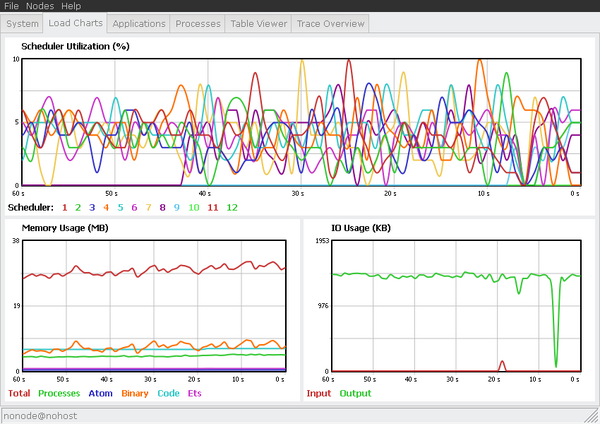
\includegraphics[scale = 0.70]{img/observerGo.jpg}
		\caption{Interface gráfica do \textit{Observer}.}
		\label{fun:fig:observer}
	\end{center}
\end{figure}

Este trabalho inclui uma nova forma de monitoramento para o barramento de serviços, esse monitoramento difere dos demais pelo modo de atuação, onde o foco é monitorar o funcionamento dos recuros que o barramento de serviços provém, desde o recurso responsável pelo registro das informações de \textit{LOG} passando pelo os recursos que executam os processos de autenticação e autorização até o recurso responsável pelo recebimento e transmissão de requisições. 

Para realizar o monitoramento foi necessária a definição de uma abordagem que permitisse o acompanhamento do funcionamento dos recursos do barramento de serviços. Nessa abordagem foi definida que as informações seriam geradas por meio do funcionamento do barramento de serviços com os seguintes passos:

\begin{itemize}
    \item Gerar dados por meio de instrumentação;
    \item Coletar e armazenar os dados oriundos da instrumentação; e
    \item Transmitir os dados para o a realização do monitoramento. 
\end{itemize}

\subsubsection{Gerar Dados por meio de Instrumentação}
O primeiro passo para realização do monitoramento foi gerar dados para o monitoramento, para isso foi utilizada uma abordagem que possibilitou a implementação no código-fonte do barramento de serviços. A abordagem inclui a criação de uma estrutura de dados e a definição de contadores numéricos, esse contadores tem a implementação simples que buscam não impactar de forma onerosa o funcionamento do barramento de serviços.

Os contadores funcionam a partir da inclusão dos métodos no código-fonte e contabilizam as informações de forma incremental, a partir do momento que os recursos do barramento de serviços são executados. A abordagem implementada e utilizada para a realização do monitoramento possibilitou o entendimento do funcionamento do barramento de serviços, e permitiu um acompanhamento completo, visto que soluções utilizadas pelo \acrshort{CPD}, acompanham o funcionamento do sistema operacional em que o barramento de serviços esta instalado ou o acompanhamento das informações de erros e regras de negócio de serviços e aplicações.      

\subsubsection{Coletar e Armazenar os Dados oriundos da Instrumentação}
O segundo passo foi implantar a funcionalidade que possibilitasse coletar e armazenar as informações geradas durante a execução do barramento do serviços. Para a realização da coleta foi necessária a inclusão de funcionalidades no código-fonte do barramento de serviços, essas funcionalidades funcionam de forma incremental a partir do funcionamento do barramento de serviços, a cada instrução executada um valor numérico é adicionado à informação de monitoramento. 

As informações coletadas são armazenadas e gerenciadas pelo agente de monitoramento que é componente responsável por gerenciar a informação referente ao monitoramento. O Agente de monitoramento possui algumas funções exclusivas, uma dessas funções é preparar a informação para a transmissão, vale lembrar que armazenar esses dados garante a integridade da informação do monitoramento.

\subsubsection{Transmitir os Dados para o a realização do Monitoramento}
Por fim, um outro passo é a transmissão dos dados de monitoramento, a transmissão dos dados é realizada após a coleta e armazenamento, o agente de monitoramento tem como responsabilidade transmitir as informações de monitoramento. Nesse trabalho a transmissão dos dados é encaminhada à uma ferramenta de monitoramento onde é possível visualizar graficamente as informações ou a emissão de notificação caso haja alguma definição para a realização do monitoramento.

Para transmitir os dados de monitoramento foi utilizada uma abordagem que permitiu a realização da transmissão de forma padronizada por meio de um protocolo de comunicação. A utilização de um protocolo possibilitou a realização da transmissão dos dados de monitoramento, assim como a integração com ferramentas de monitoramento que utilizam o protocolo \acrshort{SNMP} como meio de comunicação.  

\vspace{10mm}
\noindent
A partir a definição da estrutura de monitoramento foi realizada a geração de dados, a coleta, o armazenamento e a transmissão dos dados para monitorar os recursos do barramento. O \acrshort{CPD} possui e utiliza abordagens de monitoramento para os sistemas e ativos de rede da \acrshort{UnB}. As aplicações e ativos de rede já são monitorados em um plataforma de monitoramento mantida e gerida pelo \acrshort{CPD}, nesse trabalho foi implementada e implantada uma solução que possibilitasse a realização de integração por meio de um protocolo de comunicação para o monitoramento dos serviços, sistemas e ativos de rede na mesma plataforma mantida pelo \acrshort{CPD}, e que permitisse apresentar o funcionamento dessas aplicações ou em casos eventuais notificar sobre possíveis falhas ou problemas. 

Diante desse cenário optou-se por definir um meio de comunicação onde a ferramenta de monitoramento, mantida e gerenciada pelo \acrshort{CPD} da \acrshort{UnB} pudesse receber as informações para a realização do monitoramento do barramento de serviços, por meio de um protocolo, neste trabalho o protocolo utilizado para a realização da comunicação e permitir a integração das ferramentas foi o protocolo \acrshort{SNMP}. 

A escolha do protocolo para a realização do monitoramento busca um meio para tentar garantir a implantação e integração das aplicações com baixo acoplamento, onde a importância é a preservar a uniformidade na comunicação das aplicações por meio de um protocolo, principalmente quando houver alguma mudança de ferramenta de monitoramento, no mercado as principais ferramentas de monitoramento se comunicam e permitem a transmissão de dados e informações por meio do protocolo \acrshort{SNMP}, ou seja independente de ferramenta o serviços de monitoramento seria facilmente plugado e configurado em ferramentas de monitoramento que utilização o protocolo \acrshort{SNMP} como meio de comunicação.      

\subsection{Instrumentação de Código}
\label{instrumentacaoErlangms}

Como descrito na seção \ref{instrumentacao} o barramento de serviços dispõe de recursos que possibilitam a implementação da instrumentação em seu código. O barramento de serviços possui  um modelo de dados implementado, essa modelo é representado por uma tabela dispões de 2 colunas, 1 que identifica, ou seja, a chave e a outra com o valor do tipo inteiro referente a chave da mesma linha, alguns exemplos de chaves(identificadores) para a criação das métricas, poderão ser visualizados na figura \ref{fun:fig:chavesContadores}. 

\begin{figure}[H]
    \begin{minted}
    [frame=lines,framesep=5mm,baselinestretch=1.0]{erlang}
    ems_auth_user_public_success
    ems_auth_user_oauth2_denied
    ems_auth_user_basic_success
    ems_auth_user_oauth2_success
    ems_auth_user_public_success
    ems_oauth2_grant_type_password
    ems_oauth2_client_credentials_denied
    ems_oauth2_grant_type_token
    \end{minted}
    \caption{Exemplo de identificadores das métricas no Erlangms.}
    \label{fun:fig:chavesContadores}
\end{figure}

Para armazenar esse registros o barramento de serviços possui uma outra tabela que possibilita o registro dos contadores com identificação, hora e data, serviço e \acrshort{URL}, para fins de histórico, o barramento de serviços possui um serviço que retorna o histórico das estatísticas armazenadas, o resultado deste serviço poderá ser visualizado na figura \ref{fun:fig:webserviceStats}. 

\begin{figure}[H]
	\begin{center}
	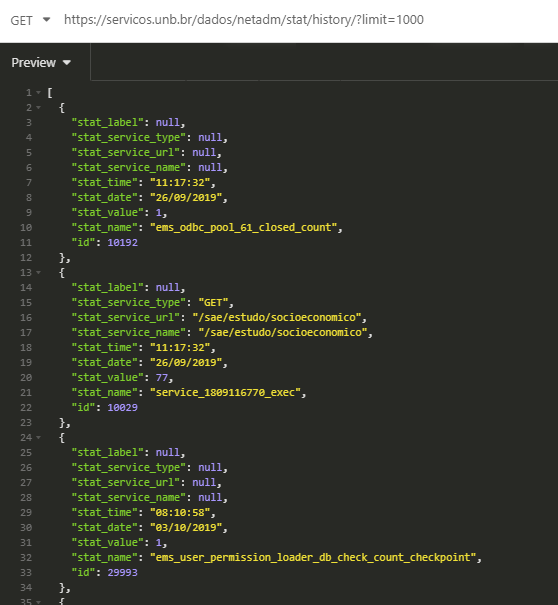
\includegraphics[scale = 0.65]{img/webserviceStats.png}
	\caption{Serviço que recupera informações históricas dos contadores do Erlangms.}
	\label{fun:fig:webserviceStats}
	\end{center}
\end{figure}

Para a realização dos registros dos contadores o barramento de serviços dispõe de funções que podem ser facilmente distribuídas pelo código fonte, especificamente em funções dos módulos do barramento de serviços, onde por meio da chave criada é possível incrementar o decrementar valores dos contadores cridos no barramento, o código da função pode ser visualizado na figura \ref{fun:fig:funcaoCounters}.   

\begin{figure}[H]
    \begin{minted}
    [frame=lines,framesep=5mm,baselinestretch=1.5]{erlang}
init_counter(Name, Value) ->
    {atomic, ok}=mnesia:transaction(fun()->
                 mnesia:write(#counter{key=Name, value=Value})end),
    ok.
inc_counter(Name)->mnesia:dirty_update_counter(counter, Name, 1).
dec_counter(Name)->mnesia:dirty_update_counter(counter, Name, -1).
current_counter(Name)->mnesia:dirty_update_counter(counter, Name, 0).
counter(Name, Inc)->mnesia:dirty_update_counter(counter, Name, Inc).
    \end{minted}
    \caption{Funções dos contadores para a Instrumentação, no Erlangms.}
    \label{fun:fig:funcaoCounters}
\end{figure}



A partir da criação dos contadores, o incremento e o decremento de seus valores é possível realização a criação das métricas. A criação das métricas é feita com utilização da aplicação Exometer, onde é possível criar métricas, definir o tipo de valor da métrica, atualizar o valor da métrica, excluir as métricas criadas, recuperar as métricas criadas e reportar métricas, no caso do \textit{report} este será feito por meio do módulo \acrshort{SNMP}. A métricas criadas na aplicação podem ser facilmente manipuladas e reportadas, graças aos métodos criados com objetivos específicos, os principais métodos utilizados nesso projeto são:
\begin{itemize}
    \item Criar métricas
    \item Excluir métricas
    \item Definir os valores de métricas
    \item Recuperar os valores de métricas
    \item Criar \textit{report} de uma métrica em SNMP
\end{itemize}

A implementação desses métodos poderão ser visualizadas na figura \ref{fun:fig:metodosExometer}, a utilização desses métodos é bem simples e permite a realização da instrumentação de maneira fácil, o que proporciona exequibilidade na personalização das informações a serem enviadas para o monitoramento, sem comprometer a eficiência do funcionamento das aplicações. 

\begin{figure}[H]
    \begin{minted}
    [frame=lines,framesep=5mm,baselinestretch=1.0]{erlang}
    % Cria uma Métrica.
    exometer:new( Name , Type ). 
    
    % Deleta uma Métrica.
    exometer:delete( Name ). 
    
    % Atualiza o valor de uma Métrica.
    exometer:update( Name , Value ). 
    
    % Recupera o valor de uma Métrica.
    exometer:get_value( Name ). 
    
    % Cria um report de uma métrica em SNMP.
    exometer_report:add_reporter( exometer_report_snmp, [] ). 
    \end{minted}
    \caption{Os métodos do Exometer utilizados no Erlangms.}
    \label{fun:fig:metodosExometer}
\end{figure}


\subsubsection{Desempenho}

Durante a realização da fundamentação teórica e do mapeamento sistemático, percebeu-se um grande número de trabalhos comentando, descrevendo e identificando o desempenho como um item preocupante e que deveria ser analisado em relação as informações geradas para o monitoramento, a transmissão dos dados de monitoramento e o funcionamento do monitoramento.  Esse item também foi analisado no projeto de modo a garantir que as informações criadas e transmitidas não comprometessem e nem onerassem a integração entre o barramento de serviços e a ferramenta de monitoramento, observando a grande quantidade de informações que podem ser geradas durante o funcionamento do barramento de serviços. 

A preocupação com  o desempenho foi minimizada após a conclusão  da implementação da instrumentação dos dados estatísticos para o monitoramento, que utilizaram um modelo de dados simples, com poucos atributos que permite após a criação da variável do contador, executar facilmente a  modificação dos valores, com isso as métricas são definidas,  criadas e utilizadas. Para que não tenha perda no desempenho, neste projeto foram implementadas funções que permitem a atualização dos contadores e a atualização das métricas ao mesmo tempo, onde primeiro executa a atualização do contador e em seguida a atualização da métrica.      

%%%%%%%%%%%%%%%%%%%%%%%%%%%%%%%%%%%%%%%%%%%%%%%%%%%%%%%%%%%%%%%




\subsection{Execução do Monitoramento}

A execução do monitoramento é inciada com a integração das aplicações, ou seja quando o barramento de serviços está em funcionamento, o agente de monitoramento está ativo, assim como a ferramenta de monitoramento está ligada e configurada em modo passivo para receber as informações que são transmitidas de modo a permitir a realização do monitoramento. Para representar a execução do monitoramento foi criado um \textit{design} que pode ser visualizado na figura \ref{fun:fig:arqtProjeto}. 

\begin{figure}[H]
	\begin{center}
	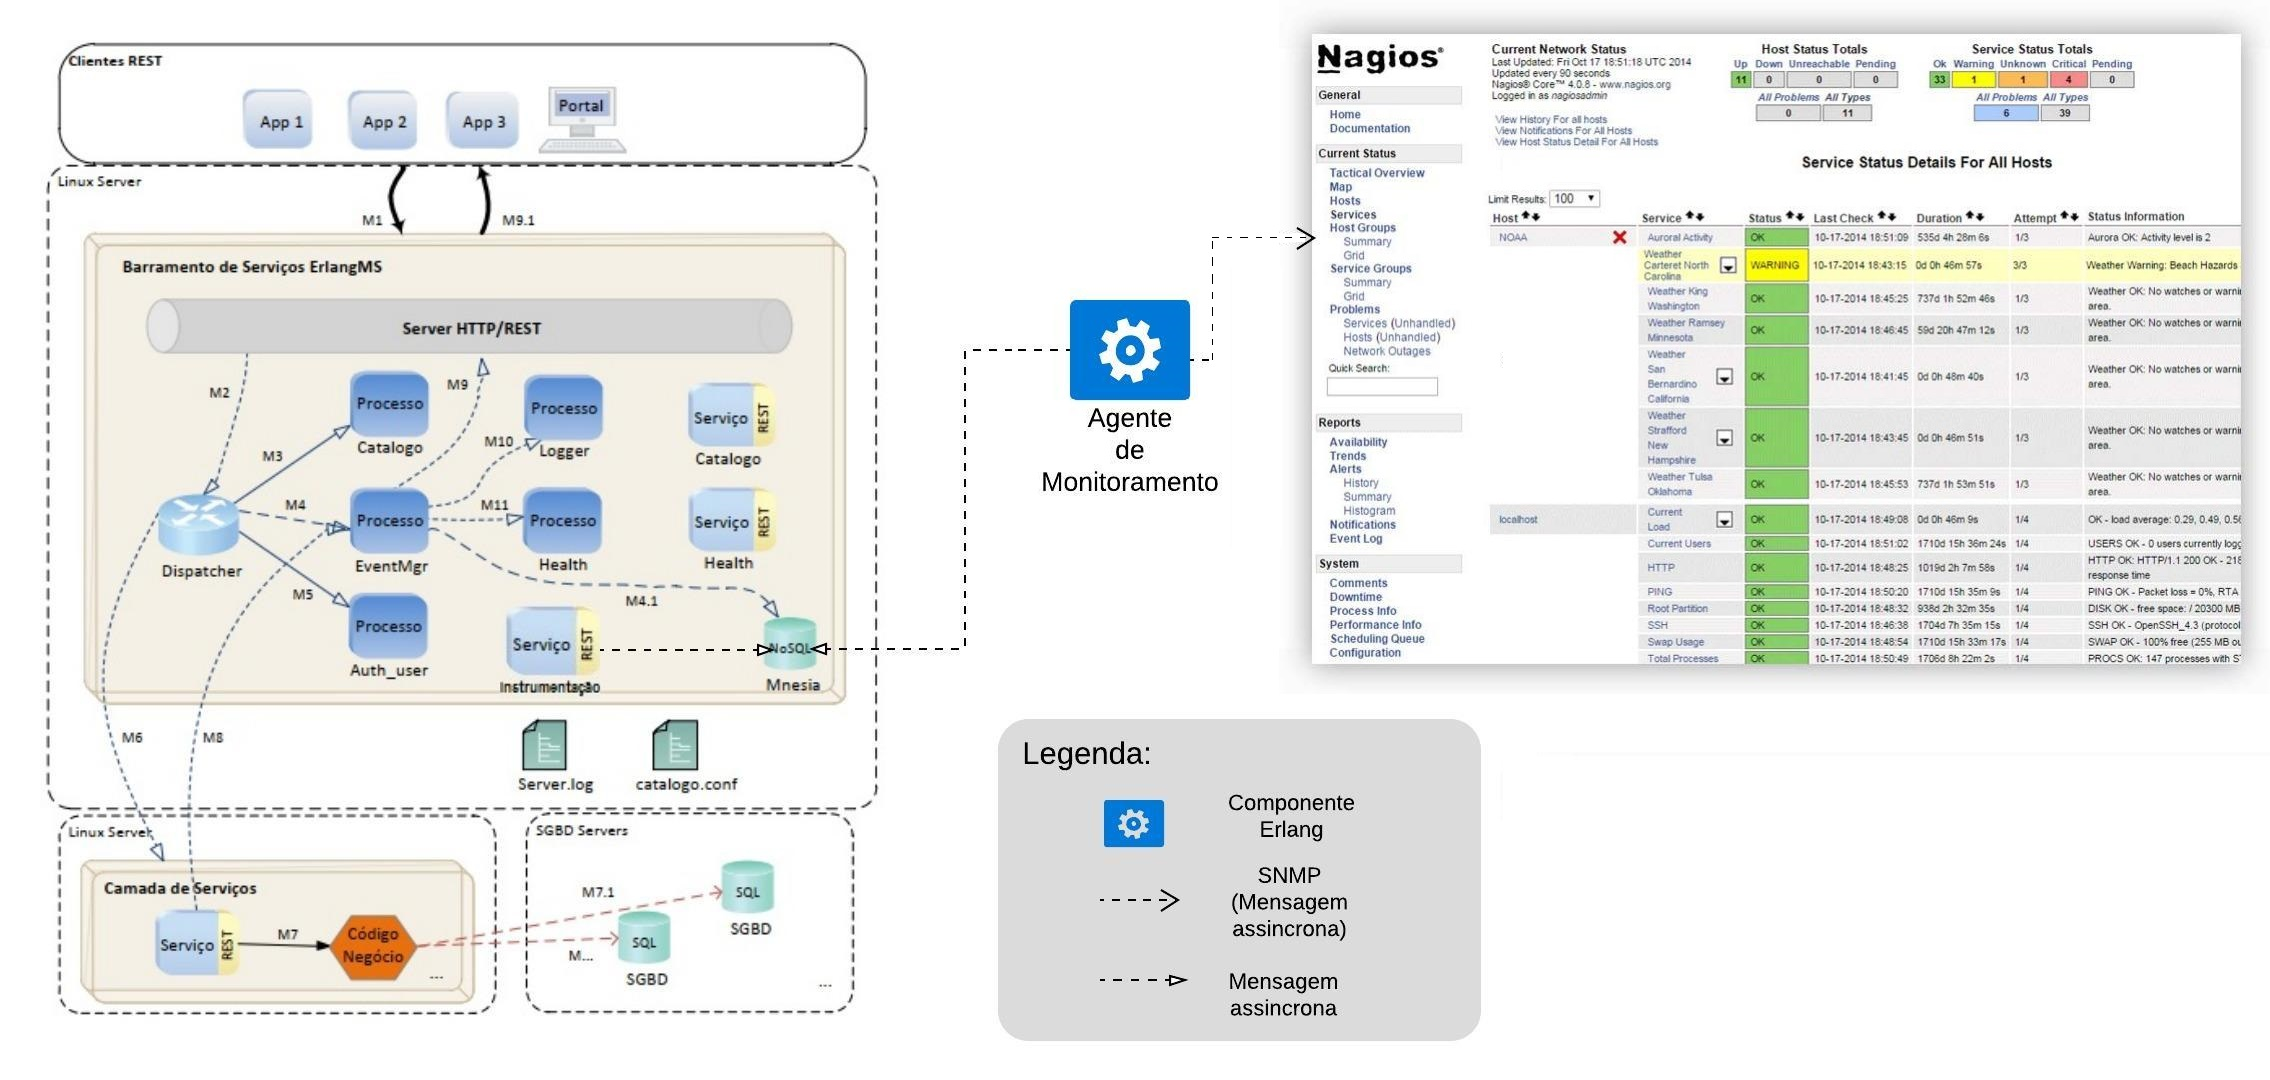
\includegraphics[scale = 0.45]{img/arqtProjeto.jpeg}
	\caption{\textit{Design} da integração das ferramentas para o monitoramento.}
	\label{fun:fig:arqtProjeto}
	\end{center}
\end{figure}


O monitoramento é realizado por meio de dados gerados por serviços provenientes do barramento de serviços, esse dados possuem identificação e valores incrementais de contagem. 

Em seu funcionamento o barramento de serviços pode incrementar ou decrementar informações de contagem dependendo do serviço utilizado, normalmente o valor é incrementado, quando o valor a ser monitorado é coletado, o mesmo é enviado ao agente de monitoramento, o agente de monitoramento tem a responsabilidade de realizar o envio dessa informação, realizando a comunicação com a ferramenta de monitoramento por meio do protocolo \acrshort{SNMP}. 

A informação transmitida poderá ser visualizada de modo personalizado e configurado na ferramenta de monitoramento, que dependendo da configuração poderá apresentar itens de serviços cadastrados com os status, \textit{"Ok"} \ para serviços que estejam funcionado normalmente, \textit{"Warning"} \  para serviços que estejam apresentando algo incomum em seu funcionamento e \textit{"Critical"} \ para serviços que estejam apresentando anormalidade ou realmente estejam indisponíveis.	 





\subsection{Execução do Agente de Monitoramento}

Para a realização da integração do barramento de serviços e a ferramenta de monitoramento por meio do protocolo \acrshort{SNMP} é utilizado um agente de monitoramento que gerencia a comunicação e transmissão dos dados que são monitorados. 

O projeto dispõem  da utilização de um agente para a coleta e transmissão desses dados, o agente é originário da aplicação Exometer que é um pacote que permite a instrumentação de aplicações desenvolvidas na linguagem de codificação Erlang, possibilitando que alguns dados do sistema sejam exportados para um grande e variado número de ferramentas de monitoramento disponíveis no mercado\cite{exometer_core}, nesse projeto diante de um dos itens do objetivo específico descrito na seção \ref{objetivos} optou-se por utilizar o modulo que permite e realizar a transmissão dos dados por meio do protocolo \acrshort{SNMP}. 

O Exometer cumpre os requisitos definidos na \acrshort{RFC} 1157 que descreve sobre os procedimentos arquiteturais de implementação e implantação do protocolo \acrshort{SNMP}. 

Os pontos fortes do Exometer que pautaram a escolha e utilização de desse \textit{software} são, a criação das \acrshort{MIBs} que são geradas dinamicamente em tempo de execução, vários tipos de criação e exportação de \textit{reports}, vários tipos de \textit{data points} que permitem selecionar o tipo de valor de uma determinada métrica, a fácil criação e utilização de métricas e o modo  acessível para a configuração do Gerente e Agente \acrshort{SNMP}, onde simplesmente você pode registrar em um dos arquivos de configuração o servidor(aplicação de monitoramento) que receberá as informações do monitoramento por meio de \textit{TRAPs} enviados pelo agente \acrshort{SNMP}. 

O Exometer foi a aplicação que permitiu a integração das aplicações de um modo dinâmico, visto que a estrutura de um arquivo MIB normalmente já vem configurada com informações específicas e estáticas o que impossibilitaria ou reduziria bastante o escopo de serviços que poderiam ser utilizados para realizar o monitoramento de serviços do barramento. 

A estrutura base do arquivo MIB utilizado pelo Exometer poderá ser visualizada na figura \ref{fun:fig:MIBSNMP} e as configurações do arquivo que gerencia o servidor de destino para receber as informações de monitoramento é apresentada na figura \ref{fun:fig:enderecoAgenteSNMP}. 

\begin{figure}[H]
    \begin{minted}
    [frame=lines,framesep=5mm,
    baselinestretch=1.5,
    fontsize=\footnotesize]{python}
    EXOMETER-METRICS-MIB DEFINITIONS ::= BEGIN
IMPORTS
    MODULE-IDENTITY, OBJECT-TYPE, NOTIFICATION-TYPE, Counter32, Counter64, 
    Gauge32, Integer32, snmpModules, experimental FROM SNMPv2-SMI
    MODULE-COMPLIANCE, OBJECT-GROUP, NOTIFICATION-GROUP FROM SNMPv2-CONF;
exometerMetricsMIB MODULE-IDENTITY
	LAST-UPDATED "201401190525Z"
	ORGANIZATION "Feuerlabs"
	CONTACT-INFO "TODO" 
	DESCRIPTION 
		"This MIB module is used for exposing dynamic exometer metrics."
	REVISION  "201401190525Z"
	DESCRIPTION 
		"The initial version"
	::= { snmpModules 1 }
exometerMetrics OBJECT IDENTIFIER ::= { experimental 7 }

-- CONTENT START

-- CONTENT END

END
    \end{minted}
    \caption{Estrutura base, arquivo MIB do Exometer.}
	\label{fun:fig:MIBSNMP}
\end{figure}



\begin{figure}[H]
    \begin{minted}
    [frame=lines,framesep=5mm,
    baselinestretch=1.5,
    fontsize=\footnotesize]{python}
   {"exometerManager",
   transportDomainUdpIpv4, 
   [127,0,0,1], 
   5000, 
   1500, 
   3, 
   "std_inform", 
   "exometerManager", 
   "exometer engine", 
   [], 
   2048}.
    \end{minted}
    \caption{Configuração do servidor de destino, para o envio de \textit{TRAPs}.}
	\label{fun:fig:enderecoAgenteSNMP}
\end{figure}


%%%%%%%%%%%%%%%%%%%%%%%%%%%%%%%%%%%%%%%%%%%%%%%%%%%%%%%%%%%%%%%

\section{Funcionamento do Protocolo SNMP}
\label{integracao_snmp}

O \acrshort{SNMP} é o protocolo utilizado para o monitoramento de dispositivos conectados em rede. O \acrshort{CPD} da \acrshort{UnB} para o monitoramento dos ativos de rede utiliza-o por meio de ferramentas que recebem informações desse protocolo, no entanto as ferramentas e informações fornecidas para o monitoramento servem apenas para o controle da infraestrutura de rede e servidores de aplicação, não gerenciando por exemplo, o funcionamento dos sistemas, serviços e também pode se dizer a ausência de verificação da saúde das aplicações. Este trabalho implementa e implanta soluções capazes de fornecer e subsidiar recursos que possibilitem o monitoramento e a integração com a ferramenta de monitoramento do \acrshort{CPD} da \acrshort{UnB} que vem durante alguns anos adotando o Nagios\textsuperscript{\textregistered} com a ferramenta de monitoramento dos seus ativos de rede, o \acrshort{SNMP} tem como característica a singularidade na comunicação o que possibilita a escolha de outras ferramentas, serviços ou aplicações que conversem em \acrshort{SNMP}. 

O funcionamento do monitoramento por meio do protocolo \acrshort{SNMP} neste trabalho é realizado pelo envio de \textit{TRAPS} a partir da coleta de informações geradas pelo barramento de serviços e enviadas pelo agente, para que o agente funcione é necessária a configuração de um gerente, o gerente funciona como a representação do cliente monitorado e o agente funciona como responsável por enviar as informações desse cliente, na figura \ref{fun:fig:agenteConfig} é apresentada a configuração do agente na aplicação e na figura \ref{fun:fig:gerenteConfig} é exposta a configuração do gerente. 

\begin{figure}[h!]
    \begin{minted}
    [frame=lines,framesep=5mm,baselinestretch=1.5]{python}
    {intAgentUDPPort, 4000}.
    {intAgentIpAddress, [127,0,0,1]}.
    {snmpEngineID, "exometer_engine"}.
    {snmpEngineMaxMessageSize, 484}.
    \end{minted}
    \caption{Arquivo de configuração do agente \acrshort{SNMP}.}
    \label{fun:fig:agenteConfig}
\end{figure}

\begin{figure}[h!]
    \begin{minted}
    [frame=lines,framesep=5mm,baselinestretch=1.5]{python}
    {port, 5000}.
    {address, [127,0,0,1]}.
    {engine_id, "manager's_engine"}.
    {max_message_size, 484}.
    \end{minted}
    \caption{Arquivo de configuração do gerente \acrshort{SNMP}.}
    \label{fun:fig:gerenteConfig}
\end{figure}

O \textit{TRAP} é um tipo de alerta ou evento que pode ser transmitido pelo protocolo, na figura \ref{fun:fig:debugTrap} é apresentada a informações de um \textit{TRAP} \acrshort{SNMP} com a verbosidade \textit{debug}. Durante a coletada das informações em tempo de execução e o envio de \textit{TRAPS} pelo agente para a ferramenta do monitoramento é necessária a instalação e configuração para de alguns \textit{plugins}, visto que o Nagios\textsuperscript{\textregistered} trabalha de forma em que é possível a realização do monitoramento ativo e passivo, como informado anteriormente este trabalho aplica o monitoramento passivo, diante desse cenário os \textit{plugins} instalados e configurados são eles:
\begin{itemize}
\item \acrfull{SNMPTT} que é um \textit{plugin} que funciona com um tradutor de \textit{TRAP} \acrshort{SNMP} com diversas opções de saída para a utilização no Nagios Core\textsuperscript{\textregistered} e o Net-SNMP\cite{nagiosCoreSNMPTT}.
\item SNMPTRAPD que é uma aplicação que funciona com o recebimento dos \textit{TRAP} que foram traduzidos pelo \acrshort{SNMPTT} \cite{net_snmptrapd}.
\end{itemize}

\begin{figure}[h!]
	\begin{center}
	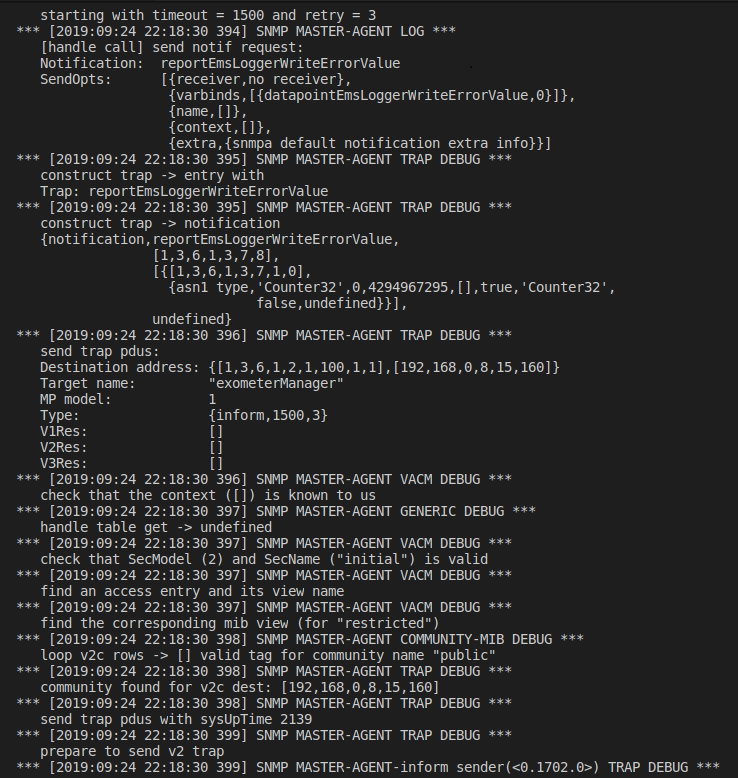
\includegraphics[scale = 0.75]{img/debugTrap.png}
	\caption{Informações do \textit{TRAP}.}
	\label{fun:fig:debugTrap}
	\end{center}
\end{figure}

Com a instalação e configuração realizada do \acrshort{SNMPTT} e SNMPTRAPD foi possível realizar a interceptação das informações enviadas pelo agente \acrshort{SNMP}, cada item com sua especifidade com por exemplo, no \acrshort{SNMPTT} é necessária a configuração das variáveis dos \acrshort{OID}s  criadas e definidas nas \acrshort{MIBs} do agente, já na configuração SNMPTRAPD é necessário definir quais os \acrshort{OID}s serão enviados à ferramenta de monitoramento e quais o tipo de informação serão enviadas, poderão ser enviadas informações dos tipos  \textit{"Ok"}, \textit{"Warning"} ,\textit{"Critical"} \ dependendo do \acrshort{OID} e da definição que pode ser facilmente configurada. Desse modo é realizada a integração das ferramentas para a execução do monitoramento, por meio do protocolo \acrshort{SNMP} a comunicação entre o barramento de serviços e o Nagios\textsuperscript{\textregistered} é praticada.  

%%%%%%%%%%%%%%%%%%%%%%%%%%%%%%%%%%%%%%%%%%%%%%%%%%%%%%%%%%%%%%%

\section{Definição das Métricas de Monitoramento}
\label{metricas_monitoramento}

Com a elaboração da integração entre o barramento de serviços e o Nagios\textsuperscript{\textregistered} foi feita a pesquisa na literatura especifica relacionada ao tema métricas de monitoramento para auxiliar a definição do que dever ser monitorado. Após a realização da pesquisa e durante a execução da configuração da ferramenta de monitoramento percebeu-se a necessidade de seguir a estrutura de configuração determinada na ferramenta de monitoramento, ao assumir essa estrutura foi possível detectar que o monitoramento deveria ser executado de um novo modo, implicando na mudança da estratégia de definição para a execução do monitoramento dos recursos do barramento de serviços. 

Como o monitoramento é realizado em modo passivo é preciso informar na configuração da ferramenta de monitoramento quais as informações serão recebidas, ou seja, mesmo o agente \acrshort{SNMP} do barramento de serviços criando os \acrshort{OID}s dinamicamente, é necessário que estes \acrshort{OID}s estejam também registrados na ferramenta de monitoramento, nesse momento  não foi possível a realização da implementação de uma solução para automatizar a configuração dinâmica dos \acrshort{OID}s na ferramenta de monitoramento, mas em um outro momento oportuno essa automatização poderá ser implementada.

Com a restrição imposta pela ferramenta de monitoramento, foi necessário a realização de um estudo no código fonte do barramento de serviços Erlangms, afim de obter informações sobre o que monitorar, a análise do barramento de serviços foi feita com alguns passos que permitiram o entendimento do funcionamento dos recursos do barramento de serviços, assim como a realização do mapeamento dos principais recursos, módulos e funções. O primeiro passo realizado foi a elaboração do \textit{design} dos recursos do barramento de serviços, este \textit{design} pode ser visualizado na figura \ref{fun:fig:ResourcesEMS}. No segundo passo foi possível identificar e escrever sobre cada recurso do barramento de serviços, a descrição dos recursos poderão ser visualizadas a seguir, são eles:

\begin{itemize}
    \item \textit{\textbf{Loaders:}}
    Responsável por carregar as configurações para o funcionamento do barramento, desde de os catálogos de serviços, passando pela identificação dos clientes até as permissões de aceso de usuários.  
    \item \textit{\textbf{HTTP(Rest Server):}}
    Responsável por realizar o funcionamento do barramento como um servidor \acrshort{REST}.
    \item \textit{\textbf{LDAP:}}
    Responsável por prover, gerenciar e autorizar acessos aos serviços por meio do barramento funcionando como um servidor REST.
    \item \textit{\textbf{ODBC:}}
    Responsável pela realização da comunicação entre os serviços do barramento com SGBDs de mercado, atualmente o barramento por meio de seus serviços realiza consultas no Postgres\textsuperscript{\textregistered} e no SQL Server\textsuperscript{\textregistered}.
    \item \textit{\textbf{Oauth2:}}
    Responsável pela autenticação e autorização de acesso aos serviços fornecidos pelo barramento
    \item \textit{\textbf{Dispatcher:}}
    Responsável pelo encaminhamento e organização das chamadas/requisições aos serviços que são executados pelo barramento.
    \item \textit{\textbf{Daemons:}}
    Responsável por gerenciar os arquivos(pid) do barramento para a execução dos serviços de forma única e confiável, sem a interrupção de seu funcionamento. 
    \item \textit{\textbf{Catalog:}}
    Responsável pela configuração, definição e funcionamento dos serviços providos pelo barramento.
\end{itemize}

\begin{figure}[h!]
	\begin{center}
	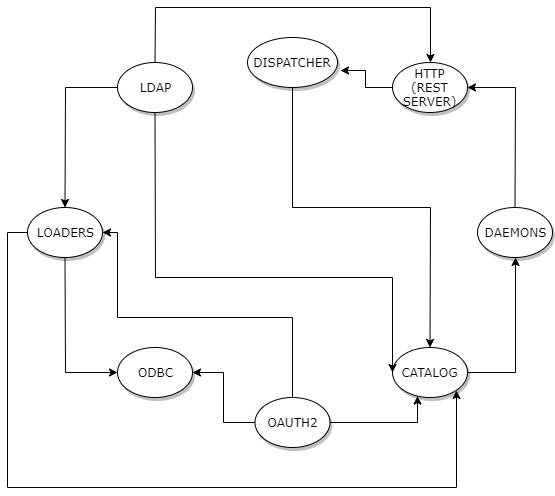
\includegraphics[scale = 0.70]{img/ResourcesEMS.png}
	\caption{Mapeamento dos recursos do barramento de serviços.}
	\label{fun:fig:ResourcesEMS}
	\end{center}
\end{figure}

Um outro passo importante foi a análise e identificação de contadores disponíveis no barramento de serviços a partir da estrutura de arquivos e diretórios, que possibilitou mapear informações de \textit{paths}, módulos e funções. Foram encontros 110 contadores registrados atualmente no barramento de serviços, o que não limita a implementação de mais contadores, os contadores estão organizados por módulos, como por exemplo, o de autenticação.  

Após a conclusão da investigação foi feita a definição das métricas por meio das informações que foram registras durante a realização da identificação dos contadores, vale salientar que as métricas foram definidas de uma forma empírica por conta da natureza da configuração e funcionamento da ferramenta de monitoramento escolhida para a execução desse trabalho, o que não significa um acoplamento alto entre as aplicações, mas sim uma forma melhor para analisar os dados enviados pelo agente \acrshort{SNMP} e recebidos pela ferramenta de monitoramento. Diante de cenário 5 métricas foram levantadas e discutidas com colaboradores da que atuam diretamente com desenvolvimento de  \textit{softwares} e colaboradores da que atuam com o monitoramento dos serviços do \acrshort{CPD} da \acrshort{UnB}, as métricas levantadas são: 

\begin{itemize}
    \item Registros do \textit{LOG} do barramento de serviços
    \item Registros de informações de Acesso (OAuth2)
    \item Registros do \textit{Dispatcher}
    \item Registros do HTTP\textit{(REST Server)}
    \item Registros de informações do LDAP
\end{itemize}

A métricas levantadas e identificadas foram definidas por apresentarem situações que poderiam contribuir diretamente na realização do monitoramento do barramento de serviços. A métrica levantada para transmissão dos dados de execução do recurso \textit{LOG} se deu pela importância de que todo o funcionamento do barramento de serviços possa ser registrado e se por algum motivo o recuros esteja registrando uma grande quantidade de falhas ou até mesmo uma exceção que o ocasione o não registro do \textit{LOG} do barramento de serviços, a ferramenta de monitoramento possa emitir notificações de alerta, esse monitoramento pode auxiliar no funcionamento do trabalho realizado por \cite{filgueirasmonitoramento} podendo respaldar alguma eventual falha no registro de \textit{LOG} do barramento de serviços, visto que o monitoramento do trabalho citado é realizado por meio de informações registradas e coletadas do arquivo de \textit{LOG} do barramento de serviços. 

Outra métrica levantada para realização do monitoramento é a que trata sobre os registros de informações de acesso por meio do protocolo OAuth2. Com a realização da transmissão dos dados dessa métrica busca-se alcançar o acompanhamento do recuros de autenticação do barramento de serviços que atualmente provém a autenticação e autorização de vários serviços e aplicações com informações provenientes de diversas bases de dados, centralizando a autenticação, o que sinaliza a necessidade de um acompanhamento em especial, visto que, uma possível falha do recurso, indisponibilidade ou um aumento expressivo de utilização do recurso possa impedir o funcionamento, impossibilitando a autenticação na aplicações. 

O registro do \textit{Dispatcher} também foi incluído como  1 das 5 métricas levantadas para a realização do monitoramento do barramento de serviços. A definição como métrica para realização da monitoramento é de suma importância para o acompanhamento do barramento de serviços, pois \textit{Dispatcher} tem como função enviar e receber as requisições de todos módulos do barramento de serviços, o que demonstra que o acompanhamento do funcionamento do \textit{Dispatcher} é indispensável. Seguindo com o levantamento das métricas, o registros do HTTP\textit{(REST Server)} também foi definido como métrica devido a execução dos operadores (GET, POST, PUT e DELETE), sua representação que no caso utiliza o formato \acrshort{JSON} e recursos (URLs) que fazem parte dos elementos mais utilizados do barramento de serviços e necessitam de acompanhamento.

Por fim, o levantamento da métrica para obtenção dos registros de informações do LDAP foi definida para que se pudesse acompanhar o funcionamento deste recurso, pois barramento de serviços realiza em seu funcionamento a autenticação de aplicações de terceiros implantadas no CPD da UnB e que utilizam o protocolo LDAP para a realização dessa autenticação, dessa forma espera-se garantir o funcionamento adequado do barramento de serviços por meio das métricas que foram levantadas, o barramento de serviços vem aumentando a disponibilização de serviços, dessa forma vale salientar sobre a importância desse acompanhamento, visto que, com o aumento dos recursos disponibilizado pelo barramento de serviços é muito grande a chance de algum falhar ou ficar indisponível e que não seja percebido ou não seja tratado imediatamente.  

Após a execução da análise das métricas levantadas foi necessário a realização da seleção e escolha das métricas a serem implantadas para e efetivação da integração entre o barramento de serviços e a ferramenta de monitoramento por meio do agente \acrshort{SNMP}. A seleção e escolha foram necessárias para que se pudesse experimentar o funcionamento da integração, pois antes da realização do monitoramento completo do barramento de serviços optou-se por implementar algumas funções que pudessem coletar informações das métricas levantadas. Das 5 métricas levantadas 3 foram escolhidas e implementadas, são elas: 

\begin{itemize}
    \item Registros do \textit{LOG} do barramento de serviços
    \item Registros de informações de Acesso (OAuth2)
    \item Registros do \textit{Dispatcher}
\end{itemize}

A escolha destas 3 métricas foi definida devido a importância do acompanhamento dos módulos mais utilizados no barramento de serviços, os registros do \textit{LOG} do barramento de serviços estão preparados para exportar e apresentar uma gama de informações podendo não facilitar a identificação de um falha ou indisponibilidade dos serviços, por isso a configuração para o registro das informações dos registros de \textit{LOG} na ferramenta de monitoramento foi escolhido. 

O motivo para escolha do registro das informações de autenticação e autorização promovidas por meio do protocolo OAuth2, foi pela quantidade crescente de disponibilização de serviços e recursos que devido a esse crescimento dificultou o acompanhamento da autenticação, por esse motivo buscou-se obter uma situação real de funcionamento do procedimento de autenticação e autorização, assim como a identificação de ataques, como por exemplo o ataque de negação de negação de serviços por meio do monitoramento. 

O funcionamento do \textit{Dispatcher} é essencial para o barramento de serviços, por ele passa todos os serviços executados pelo barramento de serviços, o \textit{Dispatcher} controla e gerencia o recebimento e envio de requisições que são executadas pelo barramento de serviços, por esse motivo acompanhar o seu funcionamento é muito importante, ainda mais com a possibilidade de emissão de notificações por meio de seu funcionamento normal e quando houver falha ou indisponibilidade, vale enfatizar que a seleção e escolhas das métricas foram realizadas por conta do modelo para realização de monitoramento que ferramenta de monitoramento selecionada propõe.   

%%%%%%%%%%%%%%%%%%%%%%%%%%%%%%%%%%%%%%%%%%%%%%%%%%%%%%%%%%%%%%%

\section{Síntese do Capítulo}
\label{sintese4}

Este capítulo apresentou o funcionamento do Monitoramento dos recursos do barramento de serviços, demonstrando a execução do monitoramento por meio da integração entre o barramento de serviços e a ferramenta de monitoramento com a utilização protocolo de monitoramento \acrshort{SNMP}, assim como a execução do agente \acrshort{SNMP} e o funcionamento do protocolo \acrshort{SNMP} no projeto. Também foram apresentadas, definidas e escolhidas a métricas mais adequadas ao funcionamento das ferramentas e a integração das aplicações para a realização do monitoramento, por fim tem-se a exposição da solução da a coleta de dados para o monitoramento por meio da instrumentação sem comprometer o desempenho durante funcionamento das aplicações e realização do monitoramento. 